%%
% This is an Overleaf template for presentations
% using the TUM Corporate Desing https://www.tum.de/cd
%
% For further details on how to use the template, take a look at our
% GitLab repository and browse through our test documents
% https://gitlab.lrz.de/latex4ei/tum-templates.
%
% The tumbeamer class is based on the beamer class.
% If you need further customization please consult the beamer class guide
% https://ctan.org/pkg/beamer.
% Additional class options are passed down to the base class.
%
% If you encounter any bugs or undesired behaviour, please raise an issue
% in our GitLab repository
% https://gitlab.lrz.de/latex4ei/tum-templates/issues
% and provide a description and minimal working example of your problem.
%%


\documentclass[
  german,            % define the document language (english, german)
  aspectratio=169,    % define the aspect ratio (169, 43)
  % handout=2on1,       % create handout with multiple slides (2on1, 4on1)
  % partpage=false,     % insert page at beginning of parts (true, false)
  % sectionpage=true,   % insert page at beginning of sections (true, false)
]{tumbeamer}


% load additional packages
\usepackage{booktabs}
\usepackage{graphicx}
\usepackage{tikz}
\usepackage{url}
\usepackage{pgfplots}
\usepackage{hyperref}
\usepackage{pmboxdraw}
\usepackage{float}
\usepackage{babel}[ngerman]
\usepackage{csquotes}[autostyle]
\usepackage[useregional]{datetime2}

% image path
\graphicspath{ {./resources/} }

% presentation metadata
\title{Übung 01: Einführung in C}
\subtitle{Grundlagenpraktikum Rechnerarchitektur}
\author{Niklas Ladurner}

\institute{\theChairName\\\theDepartmentName\\\theUniversityName}
\date{\DTMdisplaydate{2024}{4}{19}{-1}}

\footline{\insertauthor~|~\insertshorttitle~|~\insertshortdate}


% macro to configure the style of the presentation
\TUMbeamersetup{
  title page = TUM tower,         % style of the title page
  part page = TUM toc,            % style of part pages
  section page = TUM toc,         % style of section pages
  content page = TUM more space,  % style of normal content pages
  tower scale = 1.0,              % scaling factor of TUM tower (if used)
  headline = TUM threeliner,      % which variation of headline to use
  footline = TUM default,         % which variation of footline to use
  % configure on which pages headlines and footlines should be printed
  headline on = {title page},
  footline on = {every page, title page=false},
}

% available frame styles for title page, part page, and section page:
% TUM default, TUM tower, TUM centered,
% TUM blue default, TUM blue tower, TUM blue centered,
% TUM shaded default, TUM shaded tower, TUM shaded centered,
% TUM flags
%
% additional frame styles for part page and section page:
% TUM toc
%
% available frame styles for content pages:
% TUM default, TUM more space
%
% available headline options:
% TUM empty, TUM oneliner, TUM twoliner, TUM threeliner, TUM logothreeliner
%
% available footline options:
% TUM empty, TUM default, TUM infoline


\begin{document}

\maketitle

\begin{frame}[c]{}{}
  \begin{center}
    \LARGE  Keine Garantie für die Richtigkeit der Tutorfolien: Bei Unklarheiten/Unstimmigkeiten
    haben VL-Folien Recht!
  \end{center}
\end{frame}

\begin{frame}[c]{Organisatorisches}{}
  \begin{itemize}
    \item Wer bin ich?
    \item Wo könnt ihr mich erreichen?
    \item Mitschriften/Folien auf meiner \href{https://home.in.tum.de/~ladu/}{Homepage}
    \item Anmerkungen zu den Hausaufgaben/Übungen
    \item Tutoriumszeiten
    \item Vertiefungen
    \item Zulip hat eine Suchfunktion :)
  \end{itemize}
\end{frame}

\begin{frame}[c]{Artemis-Hausaufgaben}{}
  \begin{itemize}
    \item Zulassung zur Projektphase nur nach Sammeln von $\ge$ 50\%
          der Punkte in den ersten 3 Wochen!
    \item Notenbonus von 0.3, falls $\ge$ 75\% der Punkte erreicht
    \item Bearbeitet ihr eine Aufgabe, werdet ihr automatisch zur Prüfung
          angemeldet (nur relevant für 5.0X)
    \item Bonuspunkte für besonders effiziente Implementierungen (Achtung: abhängig
          vom Testserver können Ausführungszeiten abweichen)
  \end{itemize}
\end{frame}

\begin{frame}[c, fragile]{The C Programming Language}{}
  \begin{itemize}
    \item C ist eine Hochsprache, aber immer noch sehr hardwarenah
    \item Wird mittels eines Compilers (bspw. \verb|gcc|) zu Assemblercode kompiliert
    \item Includes werden in den Programmcode hineinkopiert (vgl. \verb|#ifndef ...|)
    \item Stack vs. Heap: Wo \verb|malloc|, wo \verb|alloca|?
    \item Größen von Datentypen \underline{implementierungsabhängig}
    \item \verb|stdint.h| für fixed-width Typen
    \item Für eine ausführliche Einführung siehe C-Primer (Link ganz am Ende)
  \end{itemize}
\end{frame}

\begin{frame}[c, fragile]{Pointer und Speicherobjekte}{}
  \begin{columns}[c]
    \begin{column}{0.5\textwidth}
      \begin{itemize}
        \item Pointer: Adresse zu einer Stelle im Speicher
        \item structs vs. unions
        \item Pointerarithmetik: Arrays
        \item Dereferenzierung: \verb|*| vs. \verb|&|
        \item Pointer zu Pointer: \verb|int **ptr|
      \end{itemize}
    \end{column}
    \begin{column}{0.5\textwidth}
      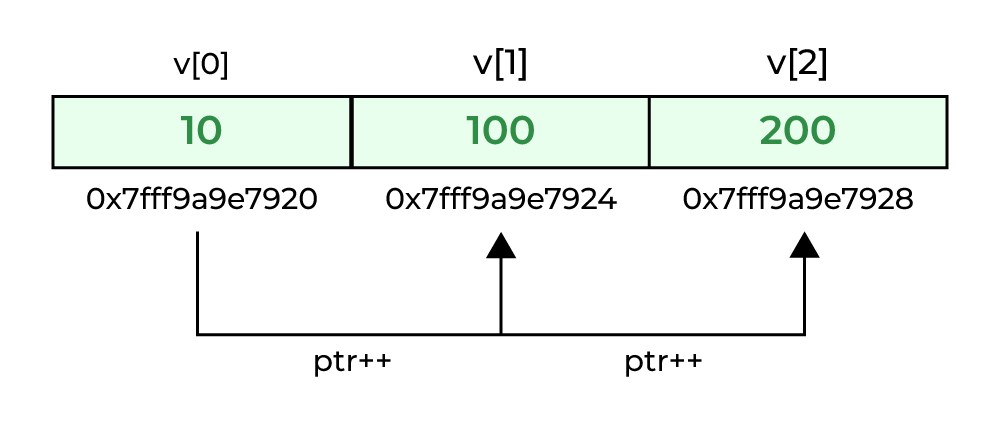
\includegraphics[width=1\textwidth]{w01_pointers.png}
      \centering
      \tiny{Quelle: \href{https://www.geeksforgeeks.org/c-pointers/}{GeeksforGeeks}}
    \end{column}
  \end{columns}
\end{frame}

\begin{frame}[c]{}{}
  \begin{center}
    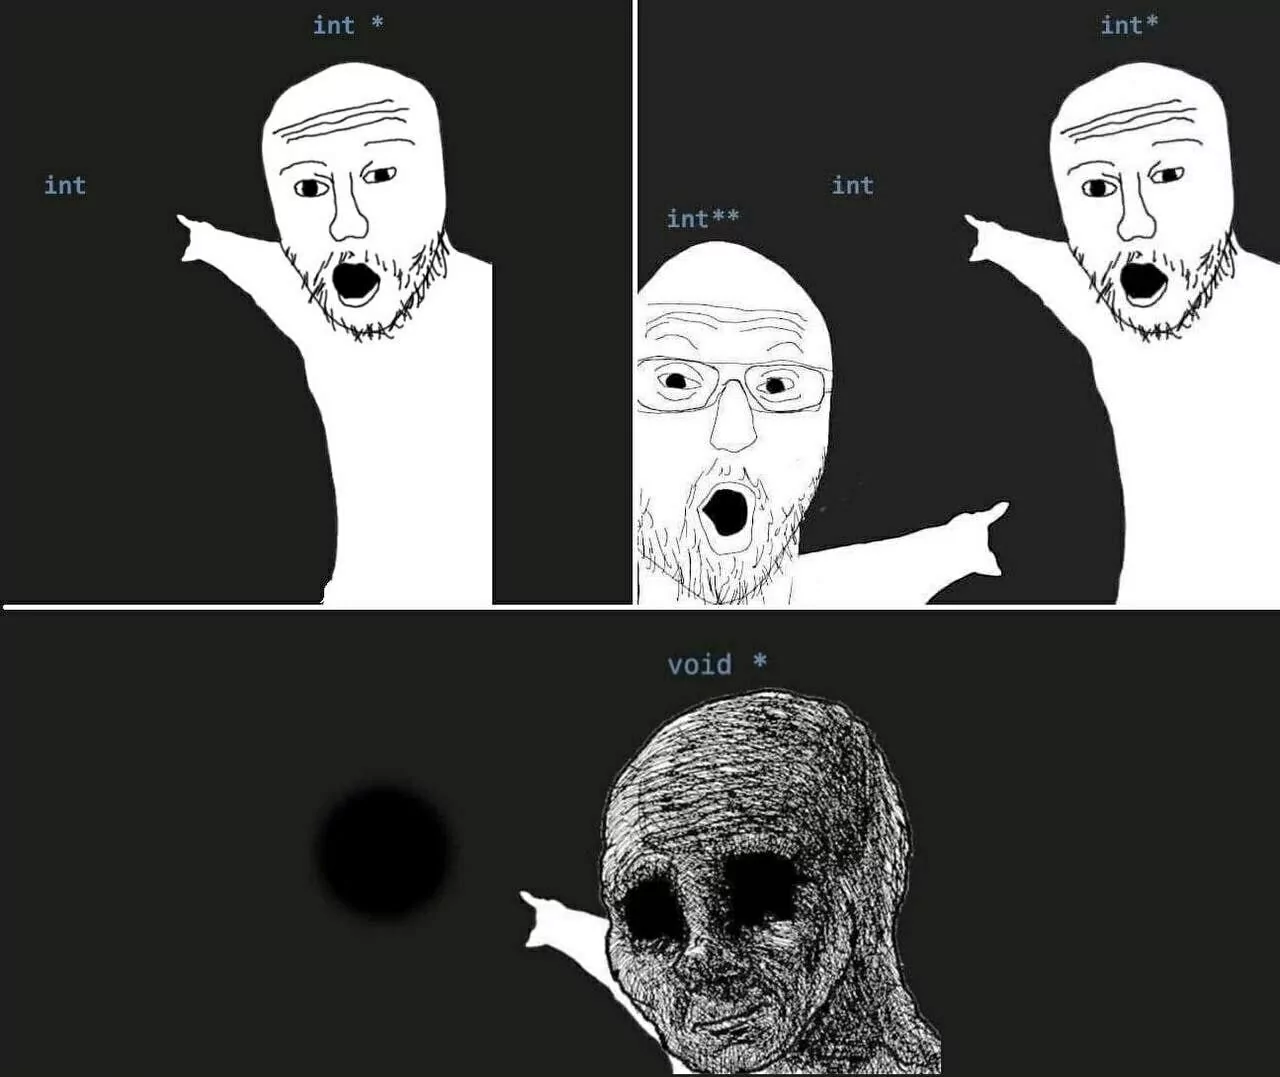
\includegraphics[height=0.9\textheight]{w01_pointers_meme.png}
  \end{center}
  \centering
  \tiny{Quelle: \href{https://programmerhumor.io/backend-memes/how-to-c-pointers/}{programmerhumor.io}}
\end{frame}

\begin{frame}[c]{}{}
  \begin{center}
    \LARGE Fragen?
  \end{center}
\end{frame}

\begin{frame}[fragile, c]{Links}{}
  \begin{itemize}
    \item Zulip: \href{https://zulip.in.tum.de/#narrow/stream/2267-GRA-Tutorium---Gruppe-20}{\enquote{GRA Tutorium - Gruppe 20}}
          bzw. \href{https://zulip.in.tum.de/#narrow/stream/2269-GRA-Tutorium---Gruppe-22}{\enquote{GRA Tutorium - Gruppe 22}}
    \item \href{https://artemis.in.tum.de/courses/329}{GRA-Artemis-Kurs}
    \item \href{https://git-scm.com/docs/gittutorial}{Git-Tutorial}, \href{https://rogerdudler.github.io/git-guide/}{alternatives Tutorial}
    \item \href{https://www.sec.in.tum.de/i20/assets/vorlesung/c_primer.pdf}{C-Primer von Jonas Pfoh}
  \end{itemize}
\end{frame}

\maketitle

\end{document}
